\documentclass[12pt]{standalone}
\usepackage{tikz}
\usetikzlibrary{arrows.meta, positioning, shapes.geometric}
\usepackage{amsmath}

\begin{document}

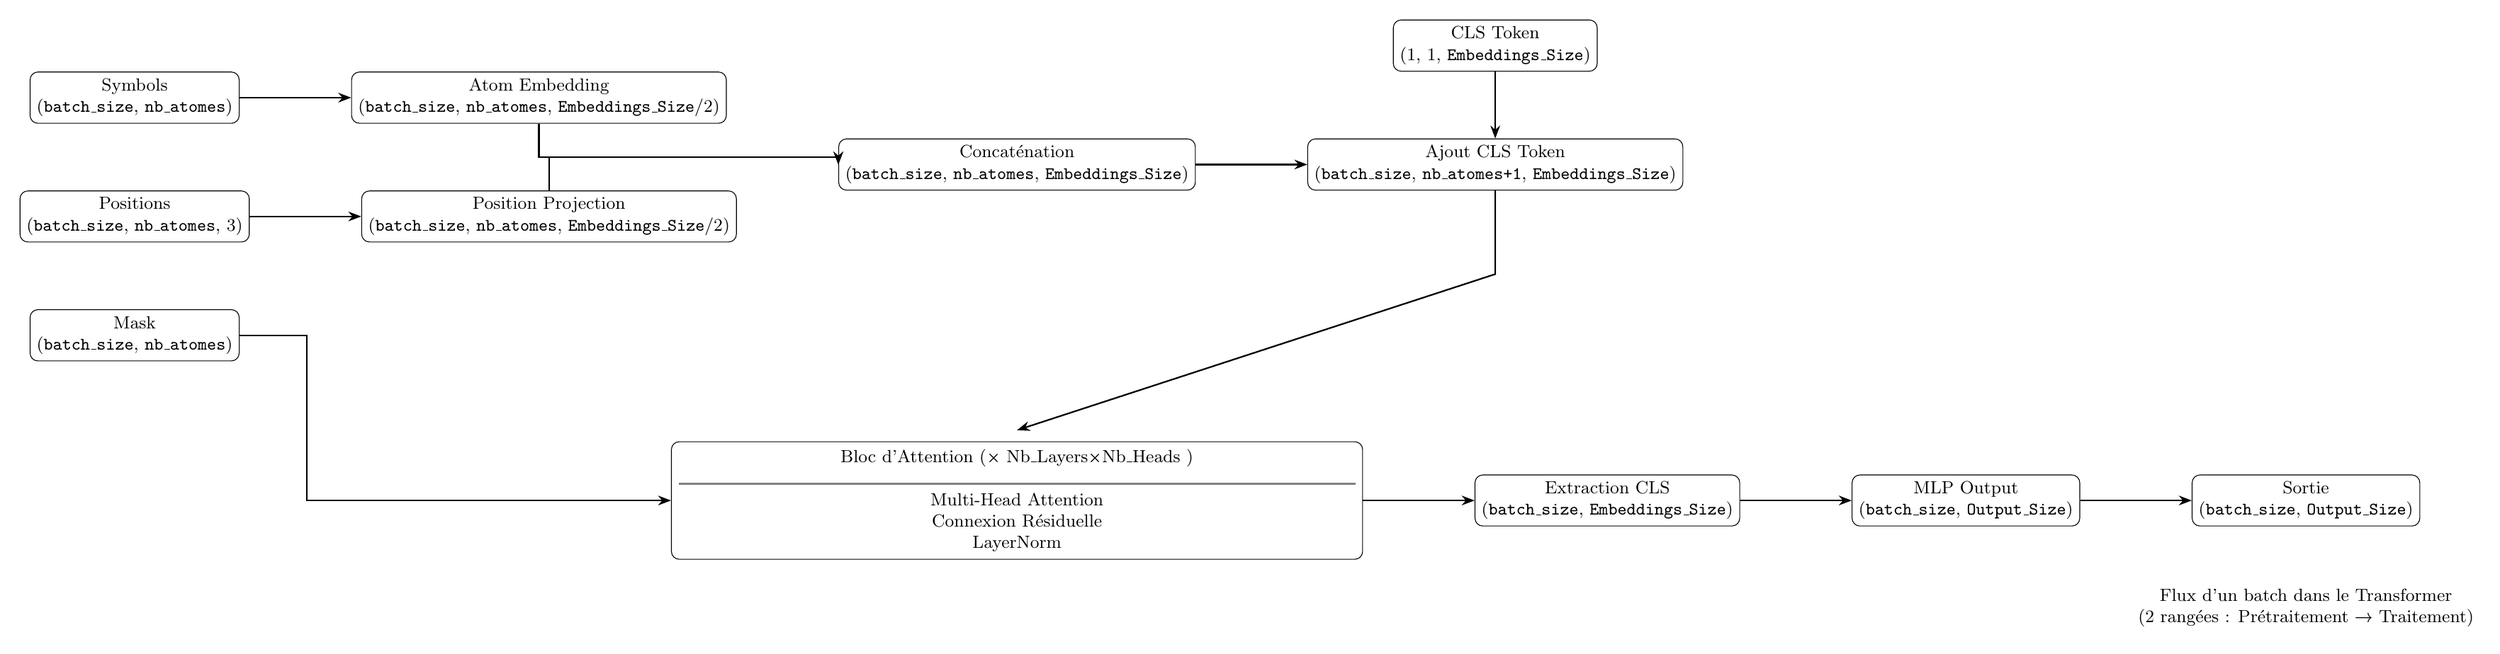
\begin{tikzpicture}[
    box/.style={rectangle, draw, rounded corners, minimum height=1.5em, minimum width=9em, align=center, font=\small},
    arrow/.style={-Stealth, thick},
    node distance=1.2cm and 2cm
]

% LIGNE 1 (entrée à CLS)
\node[box] (symbols) {Symbols\\(\texttt{batch\_size}, \texttt{nb\_atomes})};
\node[box, below=1.2cm of symbols] (positions) {Positions\\(\texttt{batch\_size}, \texttt{nb\_atomes}, 3)};
\node[box, below=1.2cm of positions] (mask) {Mask\\(\texttt{batch\_size}, \texttt{nb\_atomes})};

\node[box, right=of symbols] (atom_emb) {Atom Embedding\\(\texttt{batch\_size}, \texttt{nb\_atomes}, \texttt{Embeddings\_Size}/2)};
\node[box, right=of positions] (pos_emb) {Position Projection\\(\texttt{batch\_size}, \texttt{nb\_atomes}, \texttt{Embeddings\_Size}/2)};

\node[box, right=of atom_emb, yshift=-1.2cm] (concat) {Concaténation\\(\texttt{batch\_size}, \texttt{nb\_atomes}, \texttt{Embeddings\_Size})};
\node[box, right=of concat] (cls) {Ajout CLS Token\\(\texttt{batch\_size}, \texttt{nb\_atomes+1}, \texttt{Embeddings\_Size})};
\node[box, above=of cls] (cls_token) {CLS Token\\(1, 1, \texttt{Embeddings\_Size})};

% LIGNE 2 (bloc attention à sortie)
\node[box, below=4.5cm of concat, minimum height=6em, minimum width=12em] (attn) {Bloc d'Attention (× Nb\_Layers×Nb\_Heads )\\\tikz[baseline]{\draw[gray, thick] (0,0) -- (\linewidth,0);}\\Multi-Head Attention\\Connexion Résiduelle\\LayerNorm};

\node[box, right=of attn] (cls_extract) {Extraction CLS\\(\texttt{batch\_size}, \texttt{Embeddings\_Size})};
\node[box, right=of cls_extract] (mlp) {MLP Output\\(\texttt{batch\_size}, \texttt{Output\_Size})};
\node[box, right=of mlp] (output) {Sortie\\(\texttt{batch\_size}, \texttt{Output\_Size})};

% FLECHES LIGNE 1
\draw[arrow] (symbols) -- (atom_emb);
\draw[arrow] (positions) -- (pos_emb);
\draw[arrow] (atom_emb.south) -- ++(0,-0.6) -| (concat.west);
\draw[arrow] (pos_emb.north) -- ++(0,0.6) -| (concat.west);
\draw[arrow] (concat) -- (cls);
\draw[arrow] (cls_token) -- (cls);

% Flèche mask → attn (modifiée)
\draw[arrow] (mask.east) -- ++(1.2,0) |- (attn.west);

% Flèche cls vers attn (en descendant proprement)
\draw[arrow] (cls.south) -- ++(0,-1.5) -- ([yshift=2mm]attn.north);

% LIGNE 2
\draw[arrow] (attn) -- (cls_extract);
\draw[arrow] (cls_extract) -- (mlp);
\draw[arrow] (mlp) -- (output);

% Légende
\node[below=1cm of output, font=\small, align=center] {
Flux d’un batch dans le Transformer\\(2 rangées : Prétraitement → Traitement)
};

\end{tikzpicture}

\end{document}